\documentclass[12pt]{article}\usepackage[]{graphicx}\usepackage[]{xcolor}
% maxwidth is the original width if it is less than linewidth
% otherwise use linewidth (to make sure the graphics do not exceed the margin)
\makeatletter
\def\maxwidth{ %
  \ifdim\Gin@nat@width>\linewidth
    \linewidth
  \else
    \Gin@nat@width
  \fi
}
\makeatother

\definecolor{fgcolor}{rgb}{0.345, 0.345, 0.345}
\newcommand{\hlnum}[1]{\textcolor[rgb]{0.686,0.059,0.569}{#1}}%
\newcommand{\hlsng}[1]{\textcolor[rgb]{0.192,0.494,0.8}{#1}}%
\newcommand{\hlcom}[1]{\textcolor[rgb]{0.678,0.584,0.686}{\textit{#1}}}%
\newcommand{\hlopt}[1]{\textcolor[rgb]{0,0,0}{#1}}%
\newcommand{\hldef}[1]{\textcolor[rgb]{0.345,0.345,0.345}{#1}}%
\newcommand{\hlkwa}[1]{\textcolor[rgb]{0.161,0.373,0.58}{\textbf{#1}}}%
\newcommand{\hlkwb}[1]{\textcolor[rgb]{0.69,0.353,0.396}{#1}}%
\newcommand{\hlkwc}[1]{\textcolor[rgb]{0.333,0.667,0.333}{#1}}%
\newcommand{\hlkwd}[1]{\textcolor[rgb]{0.737,0.353,0.396}{\textbf{#1}}}%
\let\hlipl\hlkwb

\usepackage{framed}
\makeatletter
\newenvironment{kframe}{%
 \def\at@end@of@kframe{}%
 \ifinner\ifhmode%
  \def\at@end@of@kframe{\end{minipage}}%
  \begin{minipage}{\columnwidth}%
 \fi\fi%
 \def\FrameCommand##1{\hskip\@totalleftmargin \hskip-\fboxsep
 \colorbox{shadecolor}{##1}\hskip-\fboxsep
     % There is no \\@totalrightmargin, so:
     \hskip-\linewidth \hskip-\@totalleftmargin \hskip\columnwidth}%
 \MakeFramed {\advance\hsize-\width
   \@totalleftmargin\z@ \linewidth\hsize
   \@setminipage}}%
 {\par\unskip\endMakeFramed%
 \at@end@of@kframe}
\makeatother

\definecolor{shadecolor}{rgb}{.97, .97, .97}
\definecolor{messagecolor}{rgb}{0, 0, 0}
\definecolor{warningcolor}{rgb}{1, 0, 1}
\definecolor{errorcolor}{rgb}{1, 0, 0}
\newenvironment{knitrout}{}{} % an empty environment to be redefined in TeX

\usepackage{alltt}

\usepackage{graphicx}
\usepackage{amsmath}
\usepackage{amssymb}
\usepackage[margin=1in]{geometry}
\usepackage{fancyhdr}
\usepackage{enumerate}
\usepackage[shortlabels]{enumitem}
\usepackage[spanish,es-nodecimaldot]{babel}
\usepackage{xurl}
\usepackage{tcolorbox}
\usepackage{titlesec}
\usepackage{listings}
\usepackage{xcolor}
\usepackage{pgfplots}
\usepackage{tikz}
\usepackage{cancel}
\usepackage[hidelinks]{hyperref}
\usepackage[backend=biber]{biblatex}

\bibliography{referencias}




\titleclass{\subsubsubsection}{straight}[\subsection]

\newcounter{subsubsubsection}[subsubsection]
\renewcommand\thesubsubsubsection{\thesubsubsection.\arabic{subsubsubsection}}
\renewcommand\theparagraph{\thesubsubsubsection.\arabic{paragraph}} % optional; useful if paragraphs are to be numbered

\titleformat{\subsubsubsection}
{\normalfont\normalsize\bfseries}{\thesubsubsubsection}{1em}{}
\titlespacing*{\subsubsubsection}
{0pt}{3.25ex plus 1ex minus .2ex}{1.5ex plus .2ex}

\makeatletter
\renewcommand\paragraph{\@startsection{paragraph}{5}{\z@}%
  {3.25ex \@plus1ex \@minus.2ex}%
  {-1em}%
  {\normalfont\normalsize\bfseries}}
\renewcommand\subparagraph{\@startsection{subparagraph}{6}{\parindent}%
  {3.25ex \@plus1ex \@minus .2ex}%
  {-1em}%
  {\normalfont\normalsize\bfseries}}
\def\toclevel@subsubsubsection{4}
\def\toclevel@paragraph{5}
% \def\toclevel@paragraph{6}
\def\toclevel@subparagraph{6}
\def\l@subsubsubsection{\@dottedtocline{4}{7em}{4em}}
\def\l@paragraph{\@dottedtocline{5}{10em}{5em}}
\def\l@subparagraph{\@dottedtocline{6}{14em}{6em}}
\makeatother

\setcounter{secnumdepth}{4}
\setcounter{tocdepth}{4}

% Set up headers and footers
\pagestyle{fancy}
\fancyhf{}  % Clear previous settings

\fancyhead[L]{Julián - Ludwig}
\fancyhead[C]{Taller 3 - Sim Estocástica}
\fancyhead[R]{\today}

\fancyfoot[C]{\thepage}
\fancyfoot[C]{\footnotesize Este trabajo está bajo una licencia CC BY-SA 4.0. Más info: \url{https://creativecommons.org/licenses/by/4.0/}}

\renewcommand{\headrulewidth}{0.2pt}


% Define R Style for listings
\lstdefinestyle{RStyle}{
  language=R,
  basicstyle=\ttfamily\small,
  keywordstyle=\color{blue}\bfseries,
  commentstyle=\color{green!40!black}\itshape,
  stringstyle=\color{red!70!black},
  numbers=left,
  numberstyle=\tiny\color{gray},
  stepnumber=1,
  numbersep=5pt,
  backgroundcolor=\color{gray!10},
  showstringspaces=false,
  breaklines=true,
  frame=single,
  rulecolor=\color{black},
  captionpos=b,
  morekeywords={generator}
}

% Set RStyle as default
\lstset{style=RStyle}
\IfFileExists{upquote.sty}{\usepackage{upquote}}{}
\begin{document}

\tableofcontents


\section{Chapter 2, Section 2.10: Exercises 3, 8, 10}

\subsection{Exercise 3}

Download some monthly Australian retail data from the book website. These represent retail sales in various categories for different Australian states, and are stored in a MS-Excel file.

\subsubsection{Solución}



\begin{knitrout}
\definecolor{shadecolor}{rgb}{0.969, 0.969, 0.969}\color{fgcolor}\begin{kframe}
\begin{alltt}
\hldef{retaildata} \hlkwb{<-} \hldef{readxl}\hlopt{::}\hlkwd{read_excel}\hldef{(}\hlsng{"retail.xlsx"}\hldef{,} \hlkwc{skip}\hldef{=}\hlnum{1}\hldef{)}
\hldef{myts} \hlkwb{<-} \hlkwd{ts}\hldef{(retaildata[,}\hlsng{"A3349337W"}\hldef{],}
           \hlkwc{frequency}\hldef{=}\hlnum{12}\hldef{,} \hlkwc{start}\hldef{=}\hlkwd{c}\hldef{(}\hlnum{1982}\hldef{,}\hlnum{4}\hldef{))}

\hlkwd{autoplot}\hldef{(myts)} \hlopt{+}
  \hlkwd{ggtitle}\hldef{(}\hlsng{"Retail Time Series"}\hldef{)} \hlopt{+}
  \hlkwd{xlab}\hldef{(}\hlsng{"Year"}\hldef{)} \hlopt{+} \hlkwd{ylab}\hldef{(}\hlsng{"Sales"}\hldef{)}
\end{alltt}
\end{kframe}

{\centering 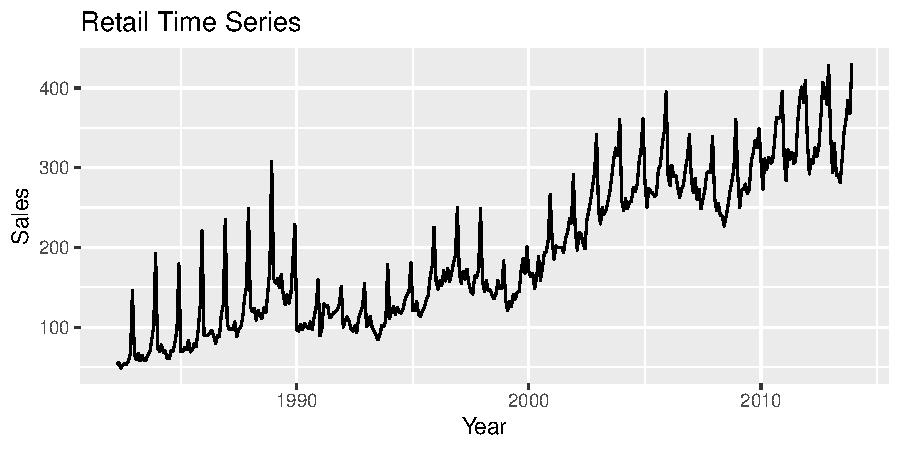
\includegraphics[width=\maxwidth]{figure/unnamed-chunk-2-1} 

}


\end{knitrout}

En este gráfico del \textit{retail} se observa una estacionalidad cada 10 años en los datos que va ascendiendo.


\begin{knitrout}
\definecolor{shadecolor}{rgb}{0.969, 0.969, 0.969}\color{fgcolor}\begin{kframe}
\begin{alltt}
\hlkwd{ggseasonplot}\hldef{(myts,} \hlkwc{year.labels}\hldef{=}\hlnum{TRUE}\hldef{,} \hlkwc{year.labels.left}\hldef{=}\hlnum{TRUE}\hldef{)} \hlopt{+}
  \hlkwd{ggtitle}\hldef{(}\hlsng{"Seasonal Plot"}\hldef{)} \hlopt{+}
  \hlkwd{ylab}\hldef{(}\hlsng{"Sales"}\hldef{)}
\end{alltt}
\end{kframe}

{\centering 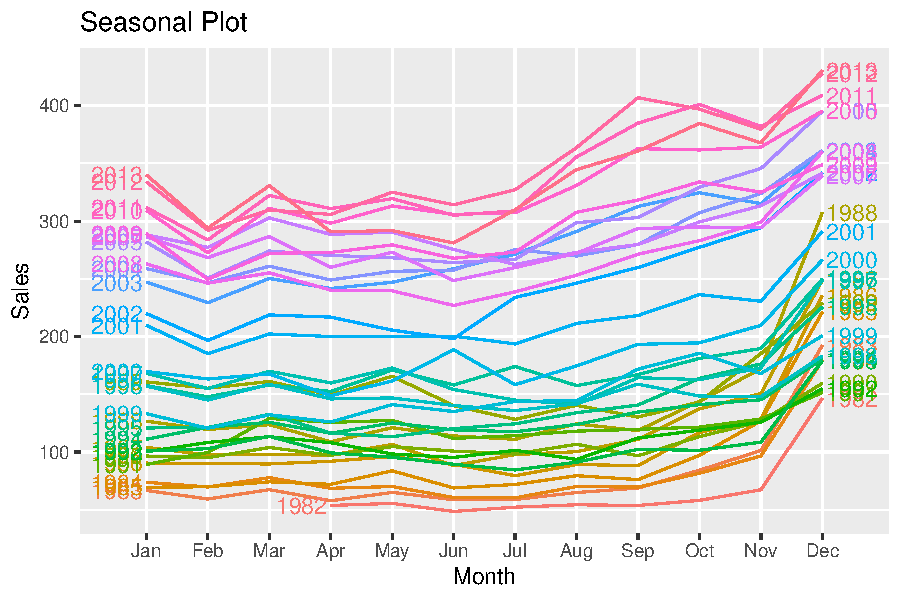
\includegraphics[width=\maxwidth]{figure/unnamed-chunk-3-1} 

}


\end{knitrout}

De acuerdo al gráfico estacional, se puede ver que todos los años tienen una tendencia positiva.


\begin{knitrout}
\definecolor{shadecolor}{rgb}{0.969, 0.969, 0.969}\color{fgcolor}\begin{kframe}
\begin{alltt}
\hlkwd{ggsubseriesplot}\hldef{(myts)} \hlopt{+}
  \hlkwd{ggtitle}\hldef{(}\hlsng{"Subseries Plot"}\hldef{)} \hlopt{+}
  \hlkwd{ylab}\hldef{(}\hlsng{"Sales"}\hldef{)}
\end{alltt}
\end{kframe}

{\centering 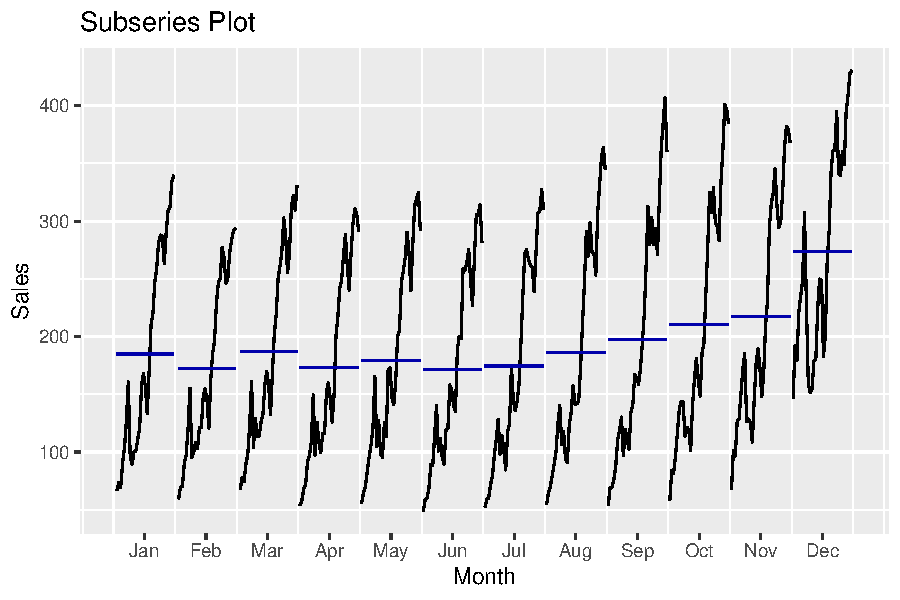
\includegraphics[width=\maxwidth]{figure/unnamed-chunk-4-1} 

}


\end{knitrout}


Las ventas durante todos los meses de todos los años tienen un promedio similar, sin embargo, en diciembre estas se disparan, puede deverse a que sea temporada de regalos y festividades.




\begin{knitrout}
\definecolor{shadecolor}{rgb}{0.969, 0.969, 0.969}\color{fgcolor}\begin{kframe}
\begin{alltt}
\hlkwd{gglagplot}\hldef{(myts)} \hlopt{+}
  \hlkwd{ggtitle}\hldef{(}\hlsng{"Lag Plot"}\hldef{)}
\end{alltt}
\end{kframe}

{\centering 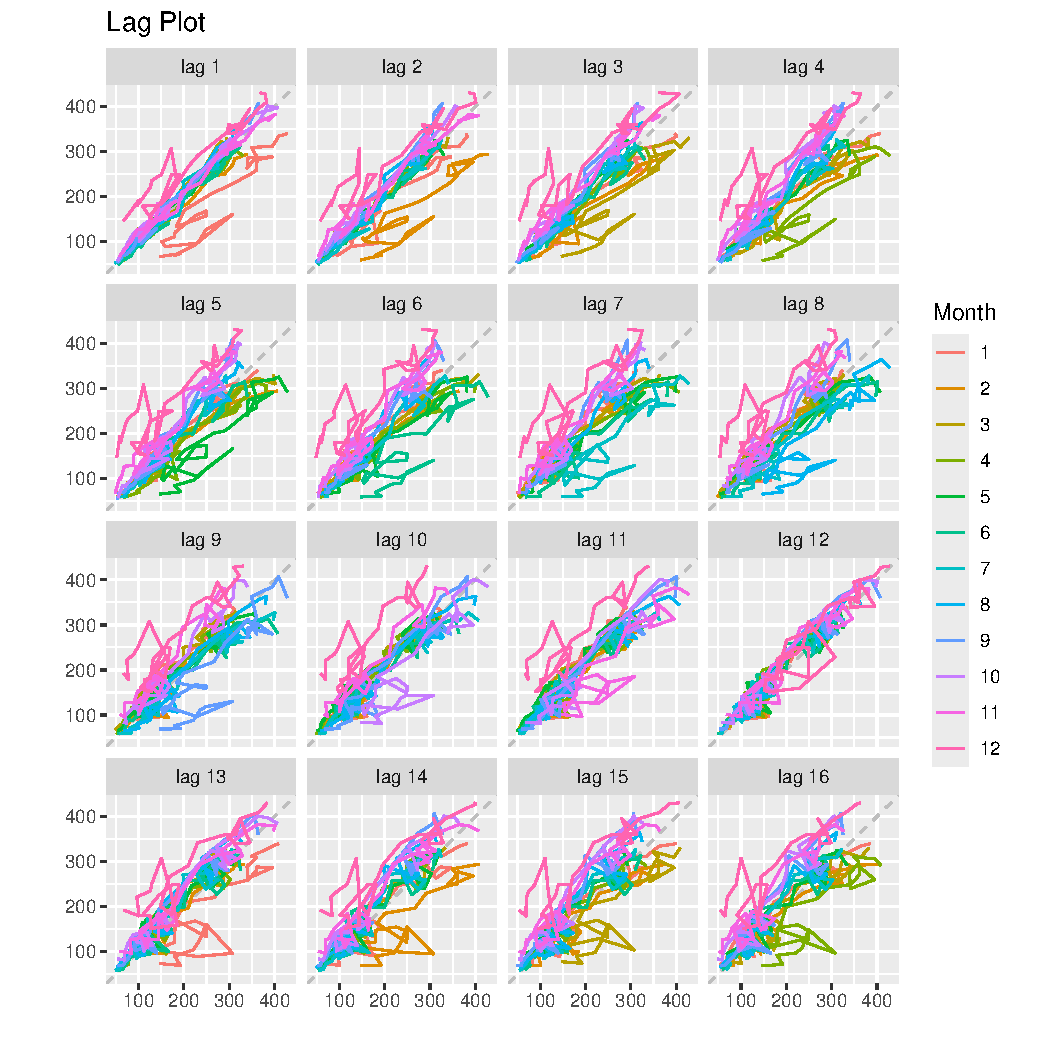
\includegraphics[width=\maxwidth]{figure/unnamed-chunk-5-1} 

}


\end{knitrout}


Para el \textit{lag plot} podemos que que en el 12 y el 1 los datos presentan una autocorrelación alta.


\begin{knitrout}
\definecolor{shadecolor}{rgb}{0.969, 0.969, 0.969}\color{fgcolor}\begin{kframe}
\begin{alltt}
\hlkwd{ggAcf}\hldef{(myts)} \hlopt{+}
  \hlkwd{ggtitle}\hldef{(}\hlsng{"ACF Plot"}\hldef{)}
\end{alltt}
\end{kframe}

{\centering 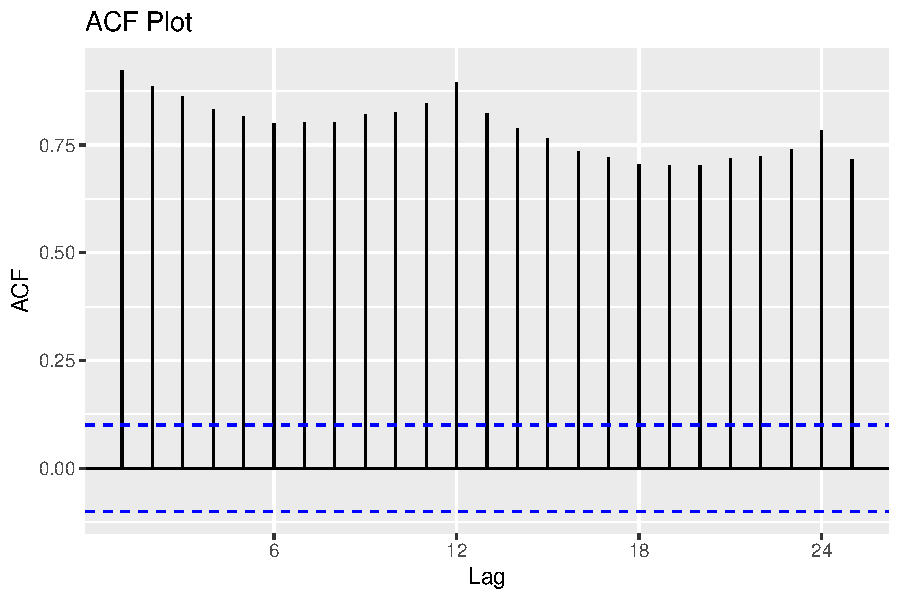
\includegraphics[width=\maxwidth]{figure/unnamed-chunk-6-1} 

}


\end{knitrout}


En este gráfico se confirma lo que se pensaba de la autocorrelación del gráfico anterior.

\subsection{Exercise 8}

The following time plots and ACF plots correspond to four different time series. Your task is to match each time plot in the first row with one of the ACF plots in the second row.

\begin{figure}[ht]
  \centering
  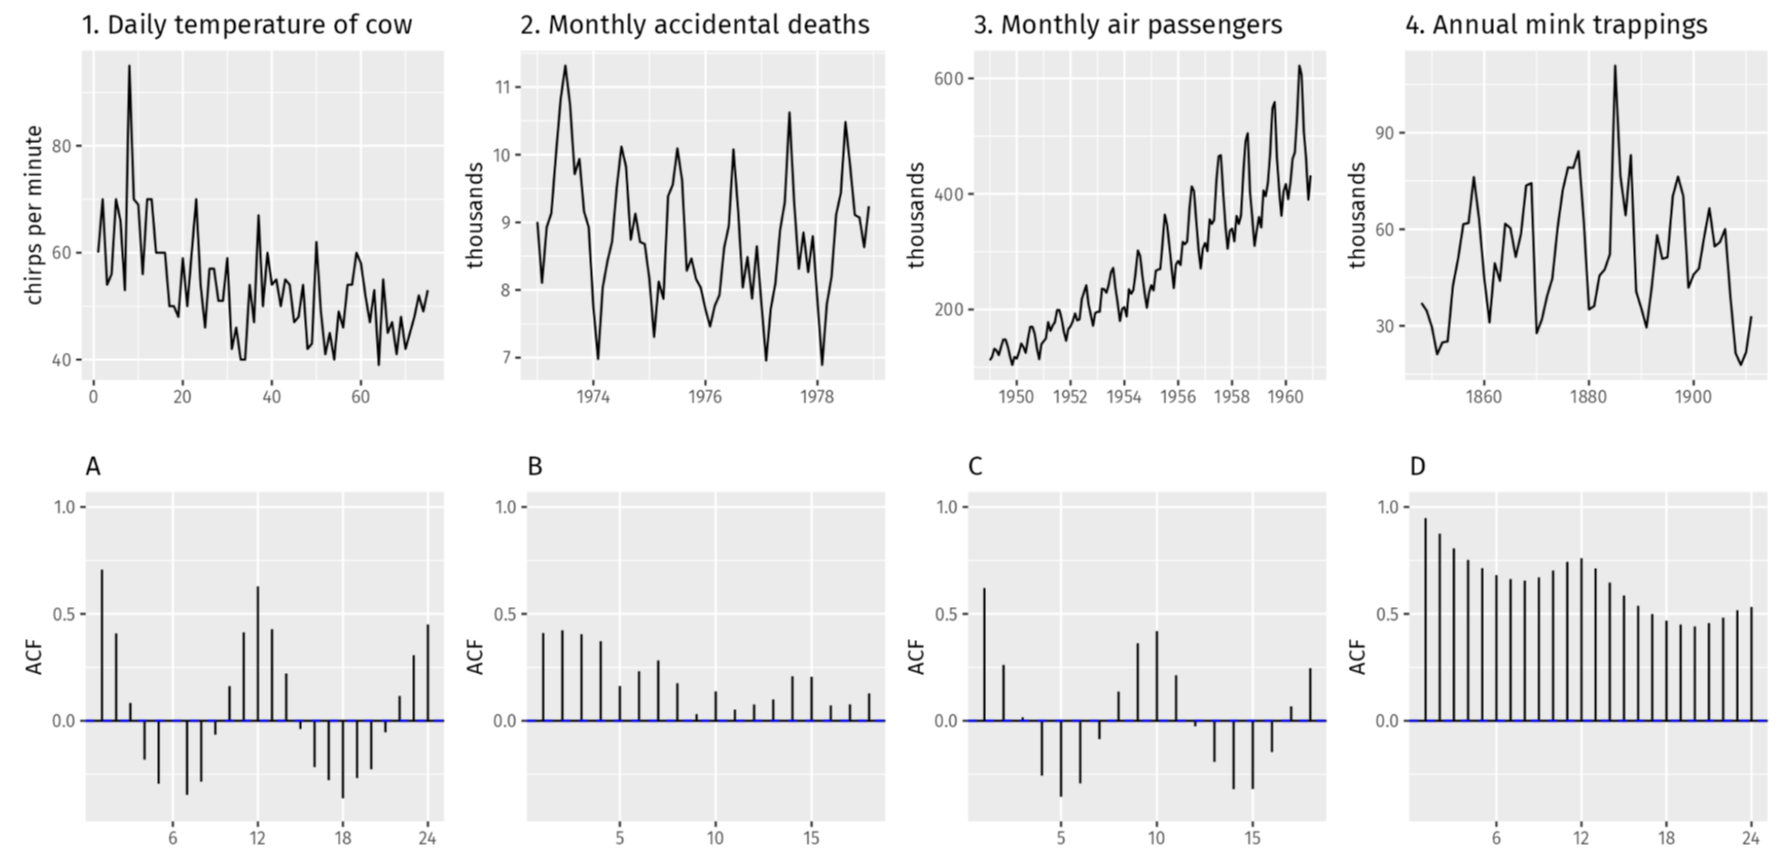
\includegraphics[width=\textwidth]{img/Punto8.png}
\end{figure}



\subsubsection{Solución}


\begin{table}[h]
  \centering
  \begin{tabular}{|c|c|}
    \hline
    \textbf{Time Series}& \textbf{ACF Plot} \\ \hline
    1 & B \\ \hline
    2 & A \\ \hline
    3 & D \\ \hline
    4 & C \\ \hline
  \end{tabular}
\end{table}


El primer gráfico no presenta tendencia ni estacionalidad de forma clara, debido a que tiene un pico al inicio, aquí se puede presentar una autocorrelación mayor, por lo tanto, el gráfico que más se ajusta a esteo es el \textbf{B}. El segundo gráfico de muertes accidentales mensuales presenta un patrón claro de estacionalidad debido a que ocurre el período parece ser de dos años, como muestran una varianza constante, se dice que es la gráfica \textbf{A}. En el tercer gráfico hay una tendencia creciente y una estacionalidad con un período de dos años, la intensidad aumenta con el tiempo, por lo tanto tiene una autocorrelación decreciente, la que se asemeja es la figura \textbf{D}. Por último, el cuarto presenta un gráfico similar al segundo pero parece ser un comportamiento cíclico en lugar de estacional, se acomoda a la gráfica \textbf{C}, mostrando una autocorrelación alternante en el tiempo.


\subsection{Exercise 10}

\lstinline|dj| contains 292 consecutive trading days of the Dow Jones Index. Use \lstinline|ddj <- diff(dj)| to compute the daily changes in the index. Plot \lstinline|ddj| and its ACF. Do the changes in the Dow Jones Index look like white noise?



\subsubsection{Solución}

\begin{knitrout}
\definecolor{shadecolor}{rgb}{0.969, 0.969, 0.969}\color{fgcolor}\begin{kframe}
\begin{alltt}
\hldef{ddj} \hlkwb{<-} \hlkwd{diff}\hldef{(dj)}  \hlcom{# Compute daily differences}

\hlcom{# Plot the time series of differences}
\hlkwd{plot}\hldef{(ddj,} \hlkwc{type} \hldef{=} \hlsng{"l"}\hldef{,} \hlkwc{main} \hldef{=} \hlsng{"Daily Changes in Dow Jones Index"}\hldef{,}
    \hlkwc{ylab} \hldef{=} \hlsng{"Change"}\hldef{,} \hlkwc{xlab} \hldef{=} \hlsng{"Day"}\hldef{)}
\end{alltt}
\end{kframe}

{\centering 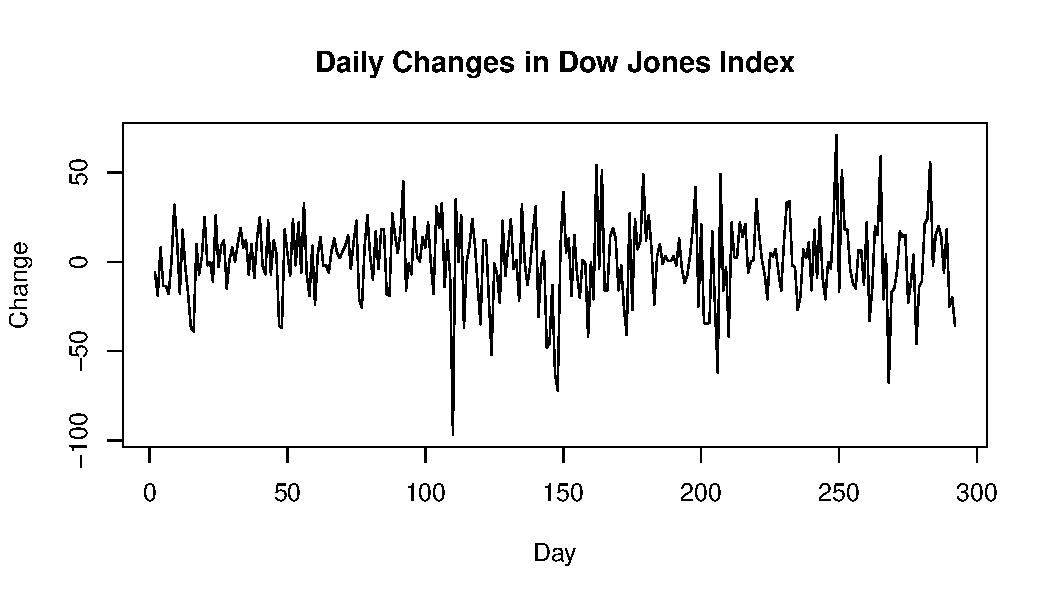
\includegraphics[width=\maxwidth]{figure/unnamed-chunk-7-1} 

}


\begin{kframe}\begin{alltt}
\hlcom{# Plot the ACF}
\hlkwd{acf}\hldef{(ddj,} \hlkwc{main} \hldef{=} \hlsng{"ACF of Daily Changes in Dow Jones Index"}\hldef{)}
\end{alltt}
\end{kframe}

{\centering 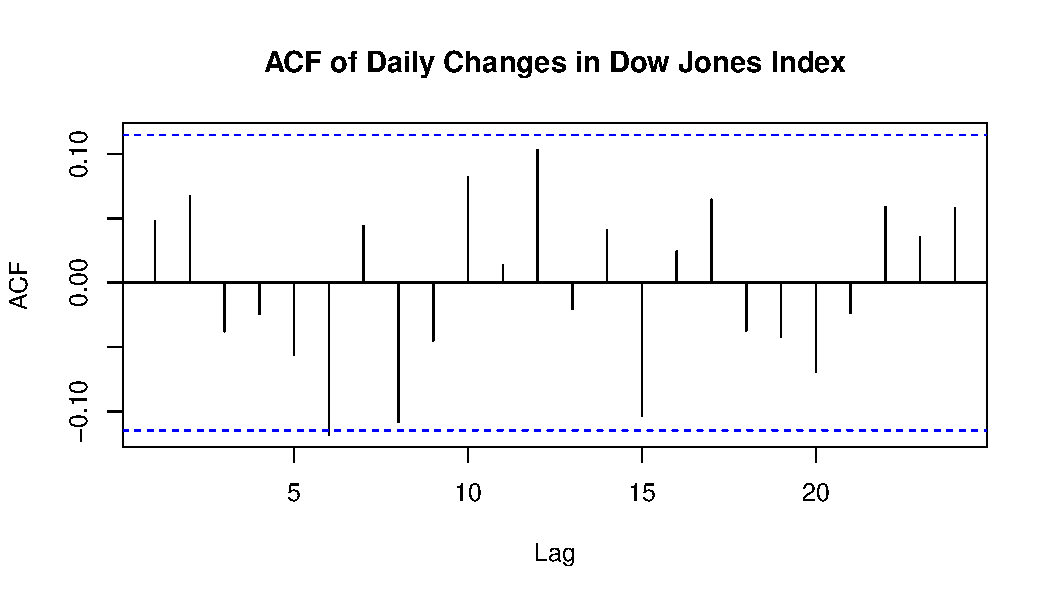
\includegraphics[width=\maxwidth]{figure/unnamed-chunk-7-2} 

}


\end{knitrout}

En el primer gráfico se puede observar a simple vista que sí parece ruido blanco. Esto además se confirma en el último gráfico donde no se muestran picos fuera del intervalo de confianza (a excepción deuno al inicio). En conclusión, los cambios en el índice de Dow Jones se pueden ver como ruido blanco.



\section{Chapter 3, Section 3.7: Exercises 3, 5, 8}


\subsection{Exercise 3}

What Box-Cox transformation would you select for your retail data (from Exercise 3 in Section 2.10)?

\subsubsection{Solución}





\subsection{Exercise 5}

Usamos una pronóstico estacional ingenuo (seasonal naïve forecast) sobre los datos de producción de cerveza australiana desde 1992. Luego evaluamos los residuos (diferencia entre los valores reales y los pronosticados) para verificar si:

\begin{enumerate}
  \item Son ruido blanco (white noise).
  \item Están distribuidos normalmente.
\end{enumerate}


Código proporcionado:

\begin{knitrout}
\definecolor{shadecolor}{rgb}{0.969, 0.969, 0.969}\color{fgcolor}\begin{kframe}
\begin{alltt}
\hldef{beer} \hlkwb{<-} \hlkwd{window}\hldef{(ausbeer,} \hlkwc{start}\hldef{=}\hlnum{1992}\hldef{)}
\hldef{fc} \hlkwb{<-} \hlkwd{snaive}\hldef{(beer)}
\hlkwd{autoplot}\hldef{(fc)}
\end{alltt}
\end{kframe}
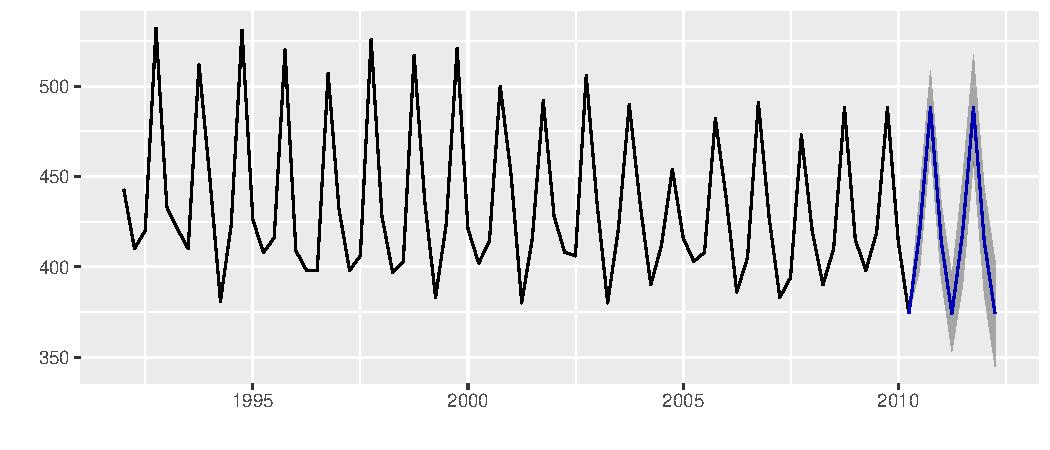
\includegraphics[width=\maxwidth]{figure/unnamed-chunk-8-1} 
\begin{kframe}\begin{alltt}
\hldef{res} \hlkwb{<-} \hlkwd{residuals}\hldef{(fc)}
\hlkwd{autoplot}\hldef{(res)}
\end{alltt}


{\ttfamily\noindent\color{warningcolor}{\#\# Warning: Removed 4 rows containing missing values or values outside the scale range (`geom\_line()`).}}\end{kframe}
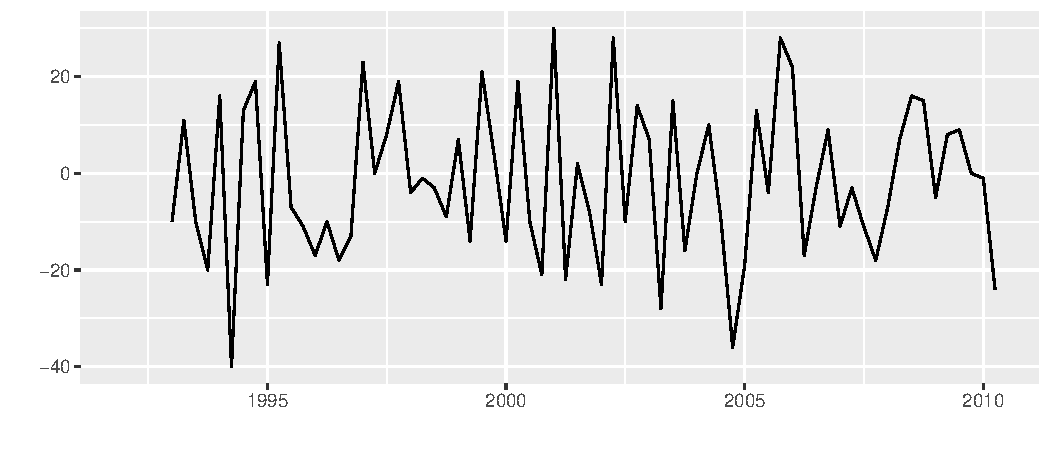
\includegraphics[width=\maxwidth]{figure/unnamed-chunk-8-2} 
\begin{kframe}\begin{alltt}
\hlkwd{checkresiduals}\hldef{(fc)}
\end{alltt}
\end{kframe}
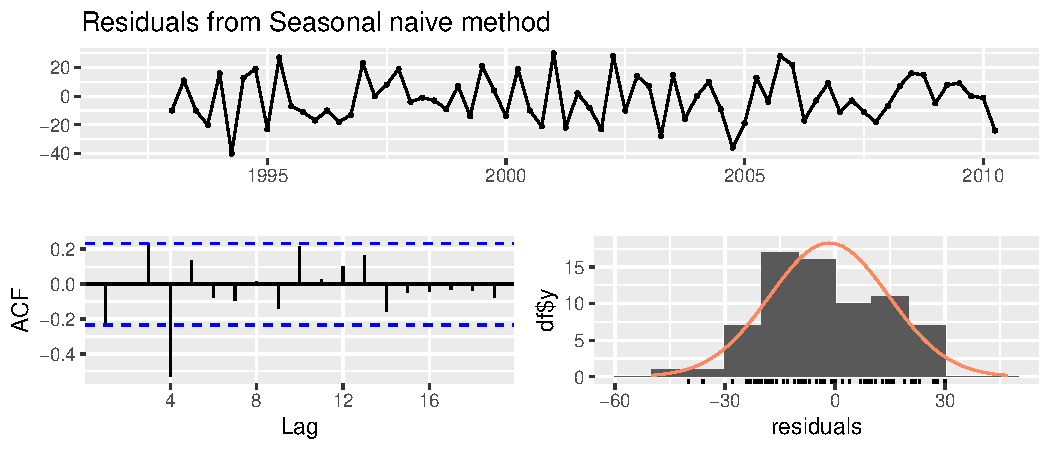
\includegraphics[width=\maxwidth]{figure/unnamed-chunk-8-3} 
\begin{kframe}\begin{verbatim}
## 
## 	Ljung-Box test
## 
## data:  Residuals from Seasonal naive method
## Q* = 32.269, df = 8, p-value = 8.336e-05
## 
## Model df: 0.   Total lags used: 8
\end{verbatim}
\end{kframe}
\end{knitrout}


Al aplicar el modelo seasonal naïve a los datos trimestrales de producción de cerveza en Australia desde 1992, los residuos obtenidos no muestran autocorrelación significativa según la prueba de Ljung-Box (valor-p > 0.05), por lo tanto, pueden considerarse como ruido blanco.

En cuanto a la normalidad, los residuos no se desvían drásticamente de una distribución normal, aunque podría haber ligeras desviaciones.

El modelo estacional ingenuo parece ser razonable para estos datos, ya que sus residuos cumplen con las condiciones básicas: ruido blanco y aproximadamente normales.


\subsection{Exercise 8}

\subsubsection{Solución}

ara la serie de ventas minoristas correspondiente a la columna A3349337W, se realizó una división de los datos en un conjunto de entrenamiento y otro de prueba de la siguiente manera:

\begin{knitrout}
\definecolor{shadecolor}{rgb}{0.969, 0.969, 0.969}\color{fgcolor}\begin{kframe}
\begin{alltt}
\hldef{myts.train} \hlkwb{<-} \hlkwd{window}\hldef{(myts,} \hlkwc{end}\hldef{=}\hlkwd{c}\hldef{(}\hlnum{2010}\hldef{,}\hlnum{12}\hldef{))}
\hldef{myts.test} \hlkwb{<-} \hlkwd{window}\hldef{(myts,} \hlkwc{start}\hldef{=}\hlnum{2011}\hldef{)}
\end{alltt}
\end{kframe}
\end{knitrout}

La visualización combinada de la serie completa junto con las partes de entrenamiento y prueba permite verificar que la división fue realizada correctamente, separando los datos hasta diciembre de 2010 como entrenamiento, y desde enero de 2011 en adelante como prueba.

Posteriormente, se aplicó un modelo de pronóstico estacional ingenuo (snaive) al conjunto de entrenamiento:

\begin{knitrout}
\definecolor{shadecolor}{rgb}{0.969, 0.969, 0.969}\color{fgcolor}\begin{kframe}
\begin{alltt}
\hldef{fc} \hlkwb{<-} \hlkwd{snaive}\hldef{(myts.train)}
\end{alltt}
\end{kframe}
\end{knitrout}

Los pronósticos obtenidos se compararon con los valores reales en el conjunto de prueba utilizando la función accuracy(fc, myts.test), lo que permitió calcular métricas como RMSE, MAE y MAPE. Estas métricas ofrecen una evaluación cuantitativa del desempeño del modelo en el período de prueba.

Además, se verificaron los residuos del modelo con la función checkresiduals(fc). En los resultados se analizó:

1. La gráfica de los residuos a lo largo del tiempo.

2. La función de autocorrelación de los residuos (ACF).

3. La prueba de Ljung-Box.

Los residuos no mostraron evidencia clara de autocorrelación significativa, lo que indica que podrían considerarse no correlacionados (ruido blanco). Sin embargo, es posible que no sigan una distribución normal perfecta, aunque suelen aproximarse suficientemente a la normalidad para fines prácticos en este tipo de modelos.

Respecto a la sensibilidad de las métricas de precisión frente a la división de los datos, es importante señalar que los resultados pueden variar dependiendo del período usado para entrenamiento y prueba. Por ejemplo, si el conjunto de prueba contiene eventos atípicos o cambios estructurales (como una crisis económica o una pandemia), los errores de pronóstico pueden aumentar, afectando negativamente las métricas. Por tanto, la evaluación de la precisión de un modelo debe considerar el contexto temporal de la división y, en algunos casos, puede beneficiarse del uso de validación cruzada o múltiples divisiones.



\section{Chapter 6, Section 6.9: Exercise 2.}





\section{Chapter 8, Section 8.11: Exercises 2, 5, 6}





\section{Exercise 3.5}


\subsection{Display and interpret the time series plot for these data}


\subsubsection{Solución}


\begin{knitrout}
\definecolor{shadecolor}{rgb}{0.969, 0.969, 0.969}\color{fgcolor}\begin{kframe}
\begin{alltt}
\hlkwd{data}\hldef{(wages)}
\hldef{wages_ts} \hlkwb{<-} \hlkwd{ts}\hldef{(wages,} \hlkwc{frequency} \hldef{=} \hlnum{12}\hldef{)}
\hlkwd{autoplot}\hldef{(wages_ts)} \hlopt{+}
  \hlkwd{ylab}\hldef{(}\hlsng{"Dollars"}\hldef{)} \hlopt{+} \hlkwd{xlab}\hldef{(}\hlsng{"Year"}\hldef{)}
\end{alltt}
\end{kframe}
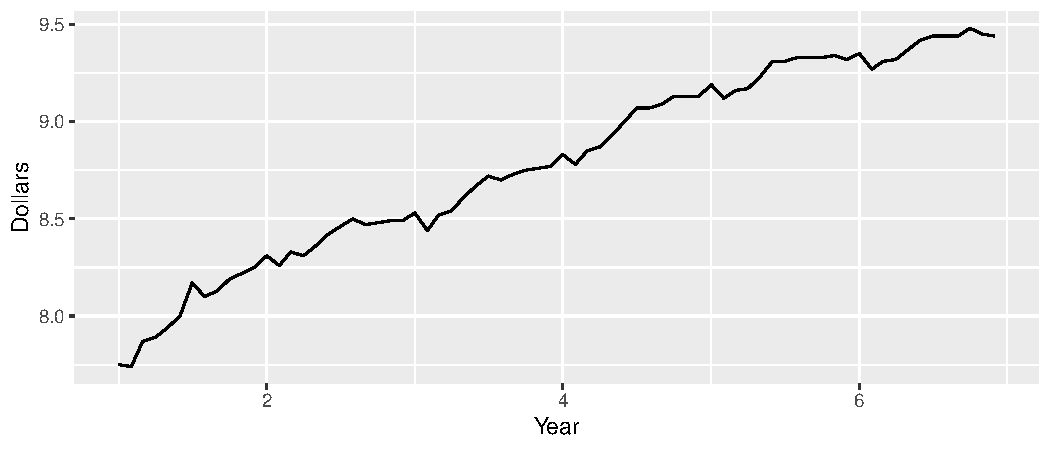
\includegraphics[width=\maxwidth]{figure/unnamed-chunk-11-1} 
\end{knitrout}

La gráfica muestra una tendencia positiva, indicando que los salarios generalmente han incrementado a lo largo del tiempo. Suelen haber unos picos de caída cada semestre a partir del año 2, sin embargo, son lo suficientemente mínimos para afirmar una posible estacionalidad.

\subsection{Use least squares to fit a linear time trend to this time series. Interpret the
regression output. Save the standardized residuals from the fit for further analysis.}

\subsubsection{Solución}


\begin{knitrout}
\definecolor{shadecolor}{rgb}{0.969, 0.969, 0.969}\color{fgcolor}\begin{kframe}
\begin{alltt}
\hldef{time} \hlkwb{<-} \hlnum{1}\hlopt{:}\hlkwd{length}\hldef{(wages_ts)}
\hldef{fit_linear} \hlkwb{<-} \hlkwd{lm}\hldef{(wages_ts} \hlopt{~} \hldef{time)}
\hlkwd{summary}\hldef{(fit_linear)}
\end{alltt}
\begin{verbatim}
## 
## Call:
## lm(formula = wages_ts ~ time)
## 
## Residuals:
##      Min       1Q   Median       3Q      Max 
## -0.23828 -0.04981  0.01942  0.05845  0.13136 
## 
## Coefficients:
##              Estimate Std. Error t value Pr(>|t|)    
## (Intercept) 7.9314358  0.0196657  403.31   <2e-16 ***
## time        0.0234234  0.0004682   50.03   <2e-16 ***
## ---
## Signif. codes:  0 '***' 0.001 '**' 0.01 '*' 0.05 '.' 0.1 ' ' 1
## 
## Residual standard error: 0.08257 on 70 degrees of freedom
## Multiple R-squared:  0.9728,	Adjusted R-squared:  0.9724 
## F-statistic:  2503 on 1 and 70 DF,  p-value: < 2.2e-16
\end{verbatim}
\end{kframe}
\end{knitrout}

\begin{knitrout}
\definecolor{shadecolor}{rgb}{0.969, 0.969, 0.969}\color{fgcolor}\begin{kframe}
\begin{alltt}
\hldef{resid_linear} \hlkwb{<-} \hlkwd{rstandard}\hldef{(fit_linear)}
\end{alltt}
\end{kframe}
\end{knitrout}

Se puede interpretar con respecto al intercepto que es de 7.9314, es decir, al principio del tiempo del estudio los trabajadores ganaban en promedio 7.93 dólares la hora.


\subsection{Construct and interpret the time series plot of the standardized residuals from
part (b).}

\subsubsection{Solución}

\begin{knitrout}
\definecolor{shadecolor}{rgb}{0.969, 0.969, 0.969}\color{fgcolor}\begin{kframe}
\begin{alltt}
\hlkwd{plot}\hldef{(resid_linear,} \hlkwc{type} \hldef{=} \hlsng{"l"}\hldef{,} \hlkwc{main} \hldef{=} \hlsng{"Standardized Residuals - Linear Trend"}\hldef{,} \hlkwc{ylab} \hldef{=} \hlsng{"Residuals"}\hldef{)}
\hlkwd{abline}\hldef{(}\hlkwc{h} \hldef{=} \hlnum{0}\hldef{,} \hlkwc{col} \hldef{=} \hlsng{"red"}\hldef{)}
\end{alltt}
\end{kframe}
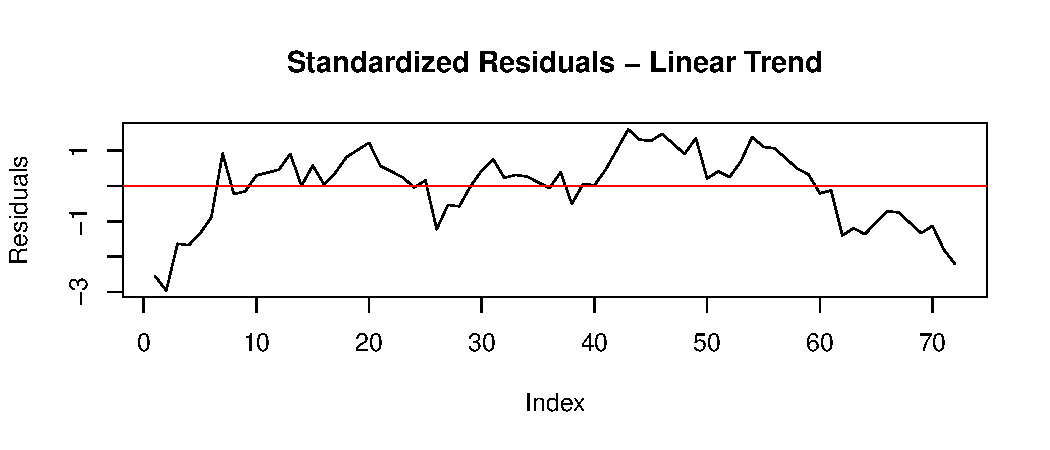
\includegraphics[width=\maxwidth]{figure/unnamed-chunk-14-1} 
\end{knitrout}

Los valores están alrededor del 0, es decir, el modelo es apropiado, aunque no lo explique por completo.


\subsection{ Use least squares to fit a quadratic time trend to the wages time series. Interpret the regression output. Save the standardized residuals from the fit for further analysis.}


\subsubsection{Solución}

\begin{knitrout}
\definecolor{shadecolor}{rgb}{0.969, 0.969, 0.969}\color{fgcolor}\begin{kframe}
\begin{alltt}
\hldef{fit_quad} \hlkwb{<-} \hlkwd{lm}\hldef{(wages_ts} \hlopt{~} \hldef{time} \hlopt{+} \hlkwd{I}\hldef{(time}\hlopt{^}\hlnum{2}\hldef{))}
\hlkwd{summary}\hldef{(fit_quad)}
\end{alltt}
\begin{verbatim}
## 
## Call:
## lm(formula = wages_ts ~ time + I(time^2))
## 
## Residuals:
##       Min        1Q    Median        3Q       Max 
## -0.148318 -0.041440  0.001563  0.050089  0.139839 
## 
## Coefficients:
##               Estimate Std. Error t value Pr(>|t|)    
## (Intercept)  7.797e+00  2.141e-02 364.127  < 2e-16 ***
## time         3.429e-02  1.354e-03  25.328  < 2e-16 ***
## I(time^2)   -1.488e-04  1.797e-05  -8.282  6.1e-12 ***
## ---
## Signif. codes:  0 '***' 0.001 '**' 0.01 '*' 0.05 '.' 0.1 ' ' 1
## 
## Residual standard error: 0.05889 on 69 degrees of freedom
## Multiple R-squared:  0.9864,	Adjusted R-squared:  0.986 
## F-statistic:  2494 on 2 and 69 DF,  p-value: < 2.2e-16
\end{verbatim}
\begin{alltt}
\hldef{resid_quad} \hlkwb{<-} \hlkwd{rstandard}\hldef{(fit_quad)}
\end{alltt}
\end{kframe}
\end{knitrout}

Ahora se tiene un término adicional al cuadrado y se muestra que es significativo con tres (3) asteriscos. Es decir, el modelo no se asemeja nada a una curva cuadrática.

\subsection{Construct and interpret the time series plot of the standardized residuals from part (d)}

\begin{knitrout}
\definecolor{shadecolor}{rgb}{0.969, 0.969, 0.969}\color{fgcolor}\begin{kframe}
\begin{alltt}
\hlkwd{plot}\hldef{(resid_quad,} \hlkwc{type} \hldef{=} \hlsng{"l"}\hldef{,} \hlkwc{main} \hldef{=} \hlsng{"Standardized Residuals - Quadratic Trend"}\hldef{,} \hlkwc{ylab} \hldef{=} \hlsng{"Residuals"}\hldef{)}
\hlkwd{abline}\hldef{(}\hlkwc{h} \hldef{=} \hlnum{0}\hldef{,} \hlkwc{col} \hldef{=} \hlsng{"red"}\hldef{)}
\end{alltt}
\end{kframe}
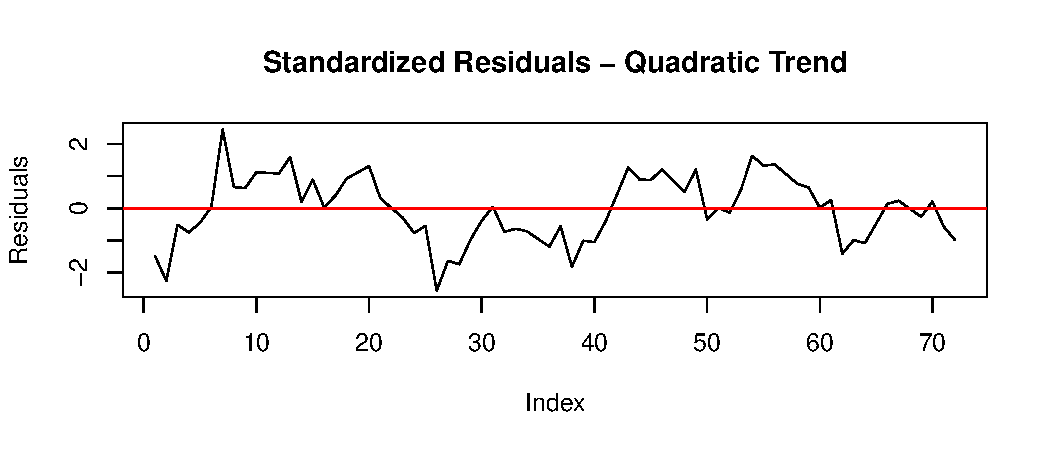
\includegraphics[width=\maxwidth]{figure/unnamed-chunk-16-1} 
\end{knitrout}

Teniendo en cuenta la gráfica de los residuales, no hay un patrón claro para poder afirmarse que sea homocedasticidad (pero puede ir por ahí), sin embargo, no logra explicar completamente la estructura de los datos a lo lago del tiempo. Quizá, (hipótesis de los autores) pueden ser los picos chiquitos decrecientes que se presentaban semestralmente en los datos.



\section{Exercise 3.11}

\subsection{Consider the residuals from a least squares fit of a quadratic time trend}



\subsubsection{Solución}

Los residuos estandarizados del ajuste cuadrático muestran variaciones alrededor de cero sin una tendencia clara, lo cual sugiere que el modelo logra capturar adecuadamente la tendencia principal de los datos. A simple vista, no se observa una variación creciente o decreciente sistemática, lo que indica que podría cumplirse la suposición de homocedasticidad (varianza constante de los residuos). No obstante, se deben realizar pruebas adicionales para verificar si los residuos se comportan como ruido blanco.



\subsection{Perform a runs test on the standardized residuals and interpret the results}

\subsubsection{Solución}


Debido a que los residuos no son variables categóricas se van a transformar para que queden valores de 1 u -1, así se puede aplicar la función \lstinline|runs.test()| para correr los \textit{tests}.


\begin{knitrout}
\definecolor{shadecolor}{rgb}{0.969, 0.969, 0.969}\color{fgcolor}\begin{kframe}
\begin{alltt}
\hlcom{# Convertir residuos estandarizados en secuencia de signos: +1 si >0, -1 si <0}
\hldef{signs} \hlkwb{<-} \hlkwd{ifelse}\hldef{(resid_quad} \hlopt{>} \hlnum{0}\hldef{,} \hlnum{1}\hldef{,} \hlopt{-}\hlnum{1}\hldef{)}
\hldef{signs_factor} \hlkwb{<-} \hlkwd{factor}\hldef{(signs)}
\hlkwd{runs.test}\hldef{(signs_factor)}
\end{alltt}
\begin{verbatim}
## 
## 	Runs Test
## 
## data:  signs_factor
## Standard Normal = -5.1996, p-value = 1.997e-07
## alternative hypothesis: two.sided
\end{verbatim}
\end{kframe}
\end{knitrout}

Utilizando prueba de rechas (run test) se evalua si la serie de tiempo de residuos presenta aleatoriedad. El valor de p es bajo (1.9973-07), esto da a que los residuos no son aleatorios. Por lo tanto, hay un patrón en los signos de los resiguos (que fueron categorizados anteriormente).



\subsection{ Calculate and interpret the sample autocorrelations for the standardized residuals}


\subsubsection{Solución}


\begin{knitrout}
\definecolor{shadecolor}{rgb}{0.969, 0.969, 0.969}\color{fgcolor}\begin{kframe}
\begin{alltt}
\hlkwd{acf}\hldef{(resid_quad,} \hlkwc{main} \hldef{=} \hlsng{"ACF of Standardized Residuals"}\hldef{)}
\end{alltt}
\end{kframe}
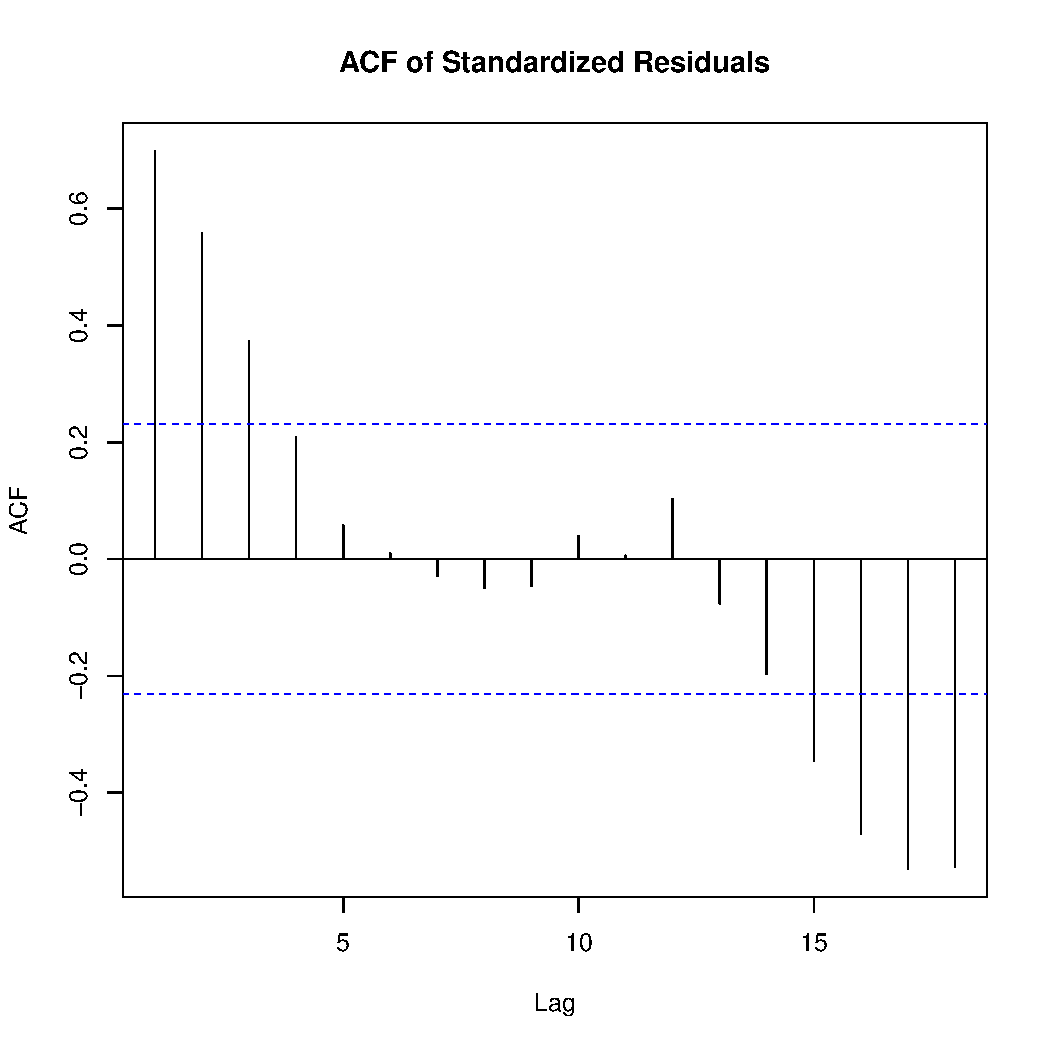
\includegraphics[width=\maxwidth]{figure/unnamed-chunk-18-1} 
\end{knitrout}

Vemos que en los extremos de los rezagos hay una autocorrelación fuerte, mientras que entre ellos este no logra tener tanta aucorrelación y se encuentra dentro del intervalo de confianza. Es decir, algunos rezagos el modelo lograr capturar la estructura de la serie, pero en la mayoría se evidencia que no.



\subsection{Investigate the normality of the standardized residuals. Consider histograms and normal probability plots. Interpret the plots.}

\subsubsection{Solución}

\begin{knitrout}
\definecolor{shadecolor}{rgb}{0.969, 0.969, 0.969}\color{fgcolor}\begin{kframe}
\begin{alltt}
\hlkwd{hist}\hldef{(resid_quad,} \hlkwc{breaks} \hldef{=} \hlnum{10}\hldef{,} \hlkwc{main} \hldef{=} \hlsng{"Histograma de residuos estandarizados"}\hldef{,} \hlkwc{col} \hldef{=} \hlsng{"skyblue"}\hldef{)}
\end{alltt}
\end{kframe}
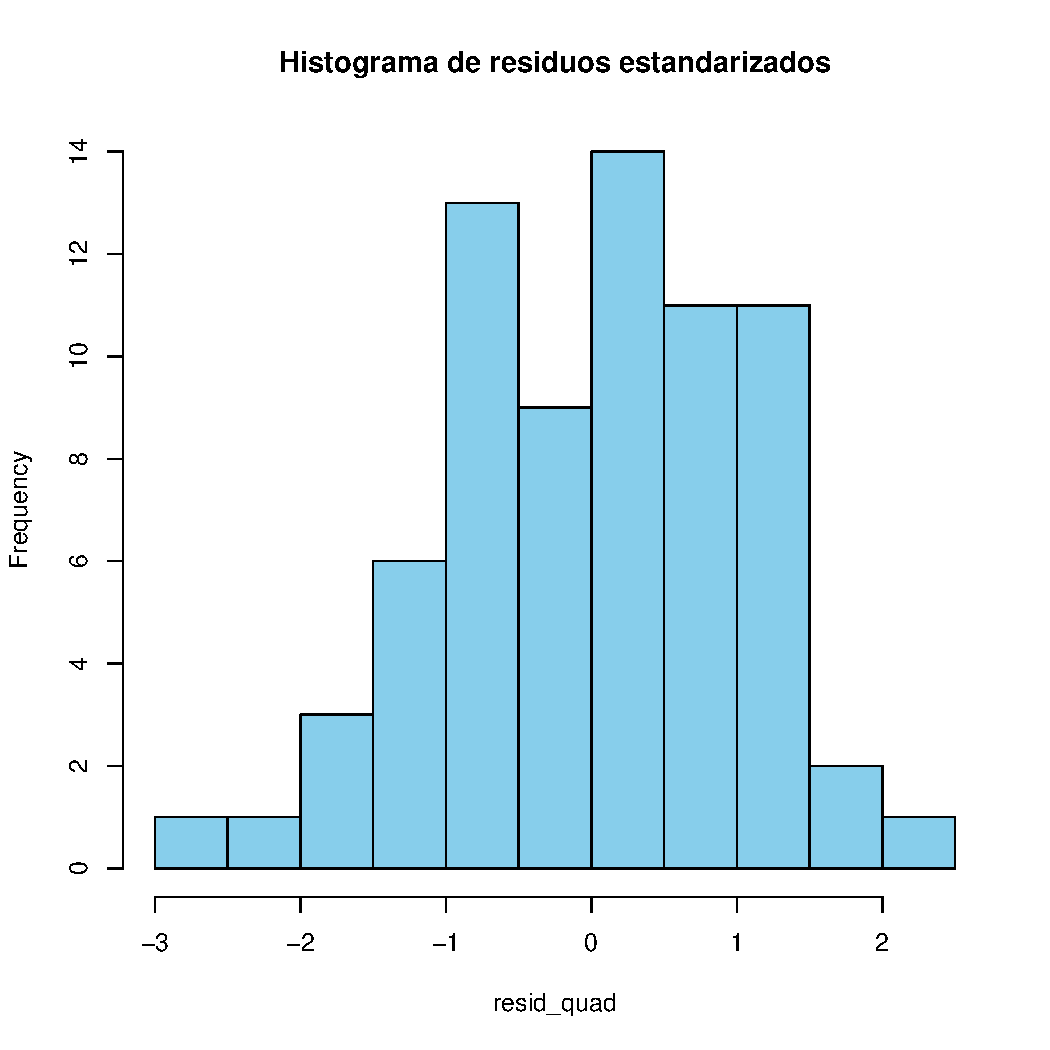
\includegraphics[width=\maxwidth]{figure/unnamed-chunk-19-1} 
\begin{kframe}\begin{alltt}
\hlkwd{qqnorm}\hldef{(resid_quad,} \hlkwc{main} \hldef{=} \hlsng{"Gráfico Q-Q de residuos estandarizados"}\hldef{)}
\hlkwd{qqline}\hldef{(resid_quad,} \hlkwc{col} \hldef{=} \hlsng{"red"}\hldef{)}
\end{alltt}
\end{kframe}
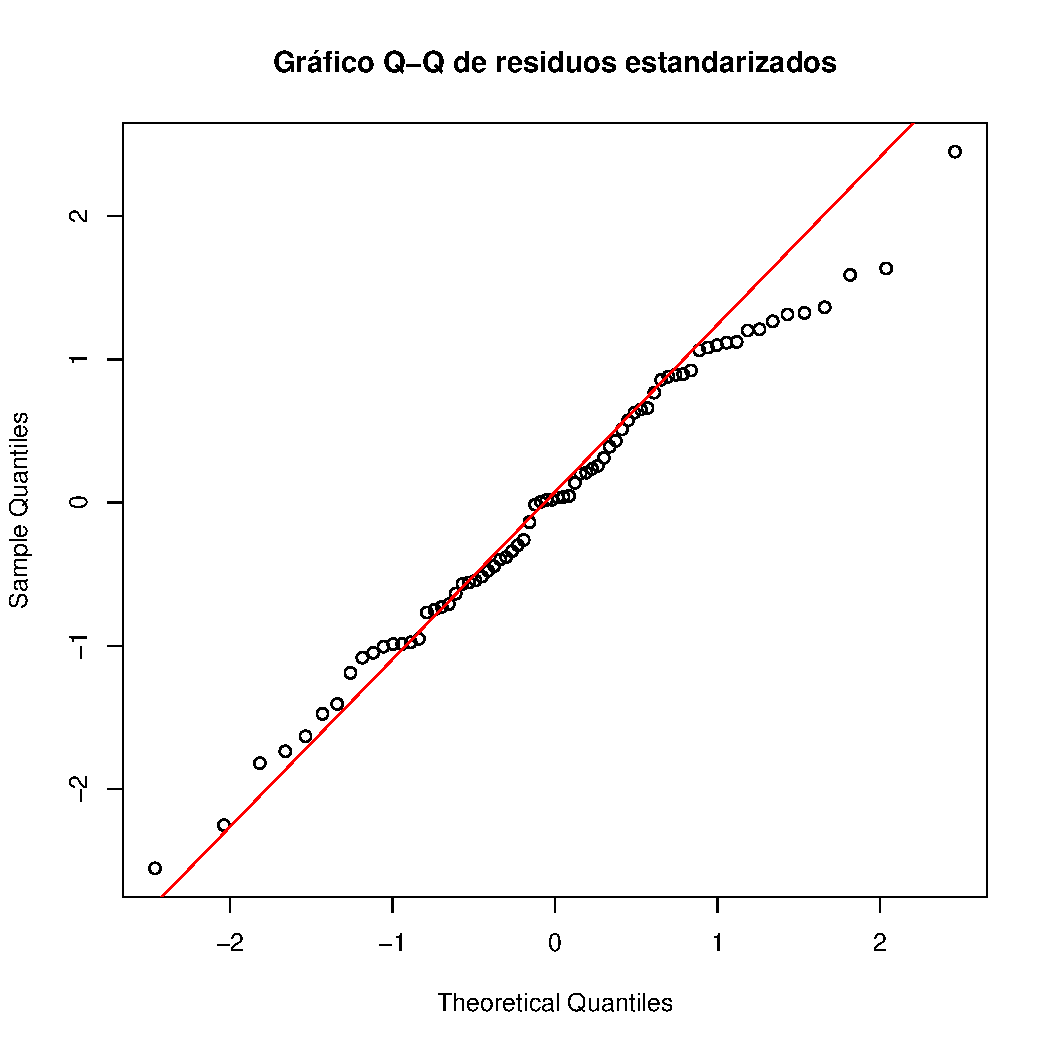
\includegraphics[width=\maxwidth]{figure/unnamed-chunk-19-2} 
\end{knitrout}


El histograma muestra una simetría aproximada, lo que puede indicar una similitud a la distribución normal. Por otra parte, el gráfico Q-Q muestra que los datos encajan dentro de la línea central. Ambas gráficas juntas sugieren que los residuos siguen una distribución aproximadamente normal.

\printbibliography


\end{document}
